%%%%%%%%%%%%%%%%%%%%%%%%%%%%%%%%%%%%%%%%%%%%%%%%%%%%%%%%%%%%%%%%%%%%%%%%%%%%%%%%
% Chapter 3: Recursos y herramientas
%%%%%%%%%%%%%%%%%%%%%%%%%%%%%%%%%%%%%%%%%%%%%%%%%%%%%%%%%%%%%%%%%%%%%%%%%%%%%%%%

%+++++++++++++++++++++++++++++++++++++++++++++++++++++++++++++++++++++++++++++++
% \section{PlayStation Camera}
% \label{3:sec:1}

% https://en.wikipedia.org/wiki/PlayStation_Camera
% https://blog.es.playstation.com/2013/10/30/ps4-las-preguntas-ms-frecuentes-que-se-te-puedan-ocurrir/#sect6

PlayStation Camera es una cámara utilizada por PlayStation 4 como accesorio. Fue
lanzada al mercado en 2013 coincidiendo con el lanzamiento de la consola, aunque
vendiendose como un accesorio a parte a un precio recomendado de 59.99\$.

\begin{wrapfigure}{l}{0.5\textwidth}
  \vspace{-20pt}
  \begin{center}
    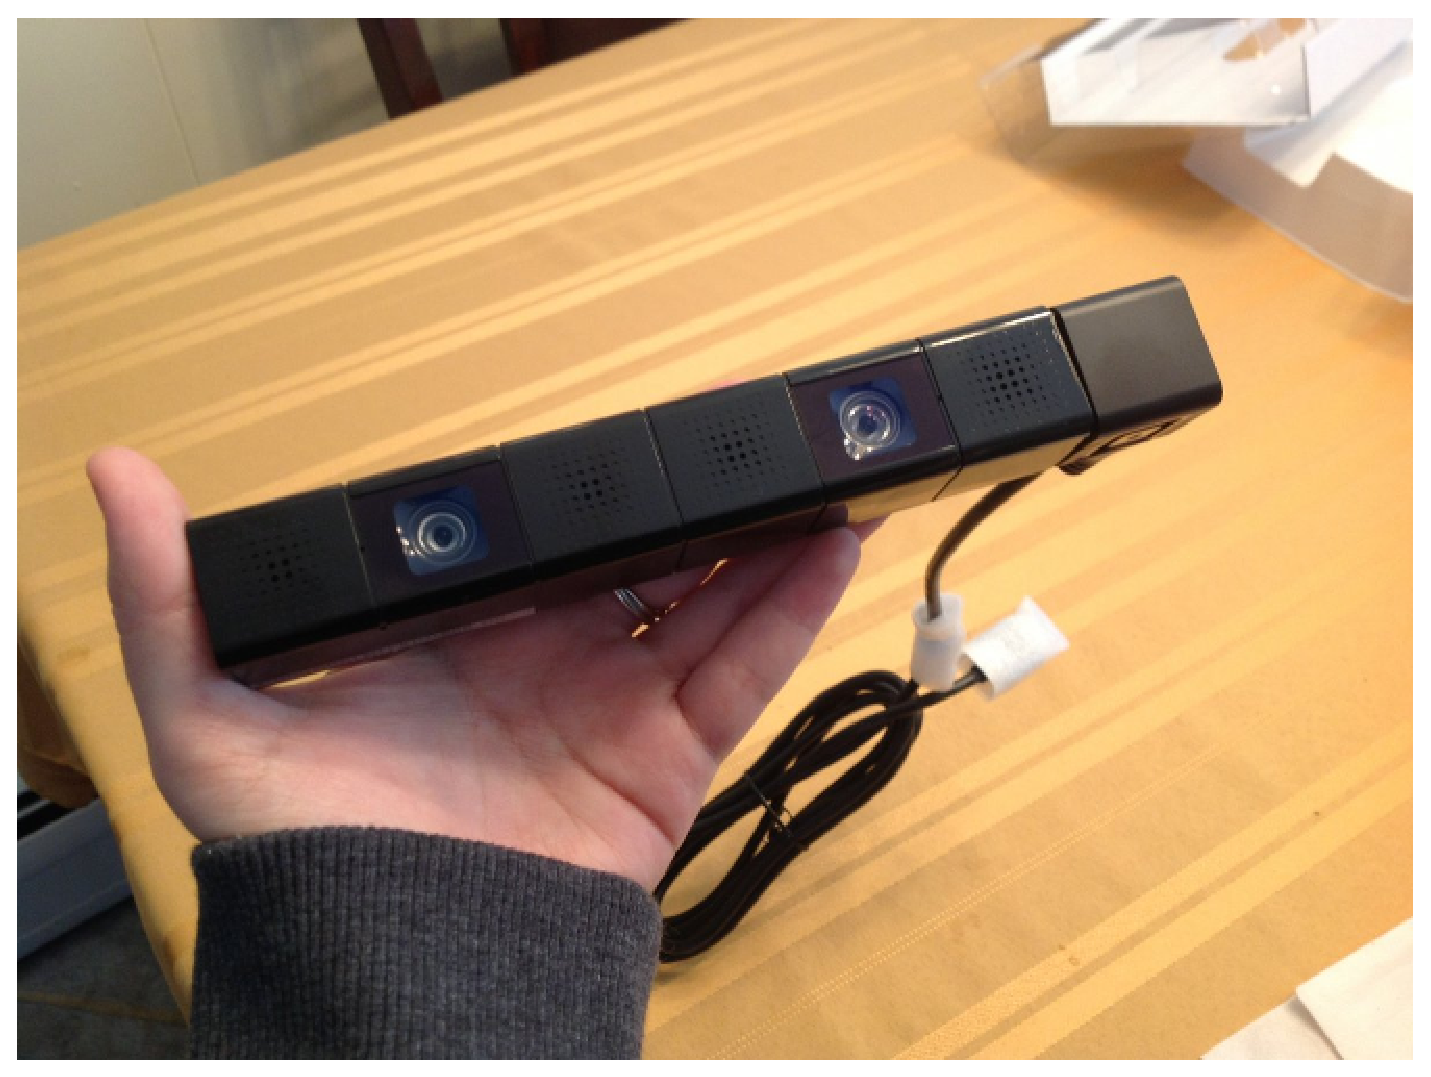
\includegraphics[width=0.48\textwidth]{images/cap3/PlaystationCamera.eps}
  \end{center}
  \vspace{-20pt}
  \caption{PlayStation Camera}
  \vspace{-10pt}
  \label{fig:PlayStation-Camera}
\end{wrapfigure}

Esta camára esta pensada para poder controlar la consola sin necesidad de
utilizar el mando tradicional. Los usuarios de PS4 pueden iniciar sesión
haciendo uso de las características de reconocimiento facial. Tambien permite
utilizar los movimientos del propio cuerpo para moverse por los menús del
sistema y utilizar la voz para realizar acciones gracias al micrófono
incorporado. Playstation Camera también es compatible con otros accesorios de
PlayStation 4 como PlayStation Move (sistema de control por movimiento) para una
navegación más precisa.

Aunque el objetivo principal de PlayStation Camera es su integración en los
vidoejuegos, para conseguir mayor inmersión: control de movimiento, comandos de
voz y tecnología de realidad aumentada.

%+++++++++++++++++++++++++++++++++++++++++++++++++++++++++++++++++++++++++++++++
\subsection{Historia}
Los orígenes de PlayStation Camera vienen desde 1999 cuando Sony empezó a
investigar sobre visión artificial y el uso de reconocimiento de gestos mediante
una cámara para incorporar esta tencnología en los videojuegos. Finalmente en
2003 se lanzaría EyeToy, una cámara que tuvo un notable éxito para PlayStation
2. En 2007, tras la salid de PlayStation 3, se lanzó al mercado una
actualización de esta cámara con el nombre de PlayStation Eye, la cual permitía
capturar imágenes a una mayor resolución y una tasa de fotogramas por segundo
superior.

Mientras que EyeToy y Playstation Eye compartían el mismo concepto, no fue hasta
el lanzamiento de Kinect por parte de Microsoft en 2010, cuando se pudo ver una
evolución real en este tipo de accesorios de entretenimiento. Kinect se basó en
una cámara RGB que contaba con sensores de profundidad, múltiples micrófonos  un
procesador independiente de la consola. Kinect permitía captura de movimiento en
3D, reconocimiento facial y reconocimiento de voz.

Kinect fue un éxito de ventas y obtuvo muchos elogios por parte de la crítica,
pero no en el plano de los vidoejuegos, si no de la investigación. Microsoft
decidió lanzar un SDK oficial para el desarrollo en Windows en base al interés
que existía, para proyectos de todo tipo.

Playstation Camera ha tomado nota de Kinect para ofrecer un producto con las
mismas ventajas de Kinect, aunque utilizando tecnología esteroscópica y
características más modestas para ser una alternativa económica a Kinect.

%+++++++++++++++++++++++++++++++++++++++++++++++++++++++++++++++++++++++++++++++
\subsection{Especificaciones técnicas}
% http://www.psdevwiki.com/ps4/PlayStation_4_Camera

PlayStation Camera cuenta con un chip OV580 encargado de sincronizar las dos
cámaras. Cada cámara cuenta con un sensor de imagen OV9713, mientras que el chip
que controla el sonido es el AK5703. La configuración inicial de la cámara se
almacena en una memoria EEPROM 4g51A.

\begin{minipage}{\linewidth}
    \centering
    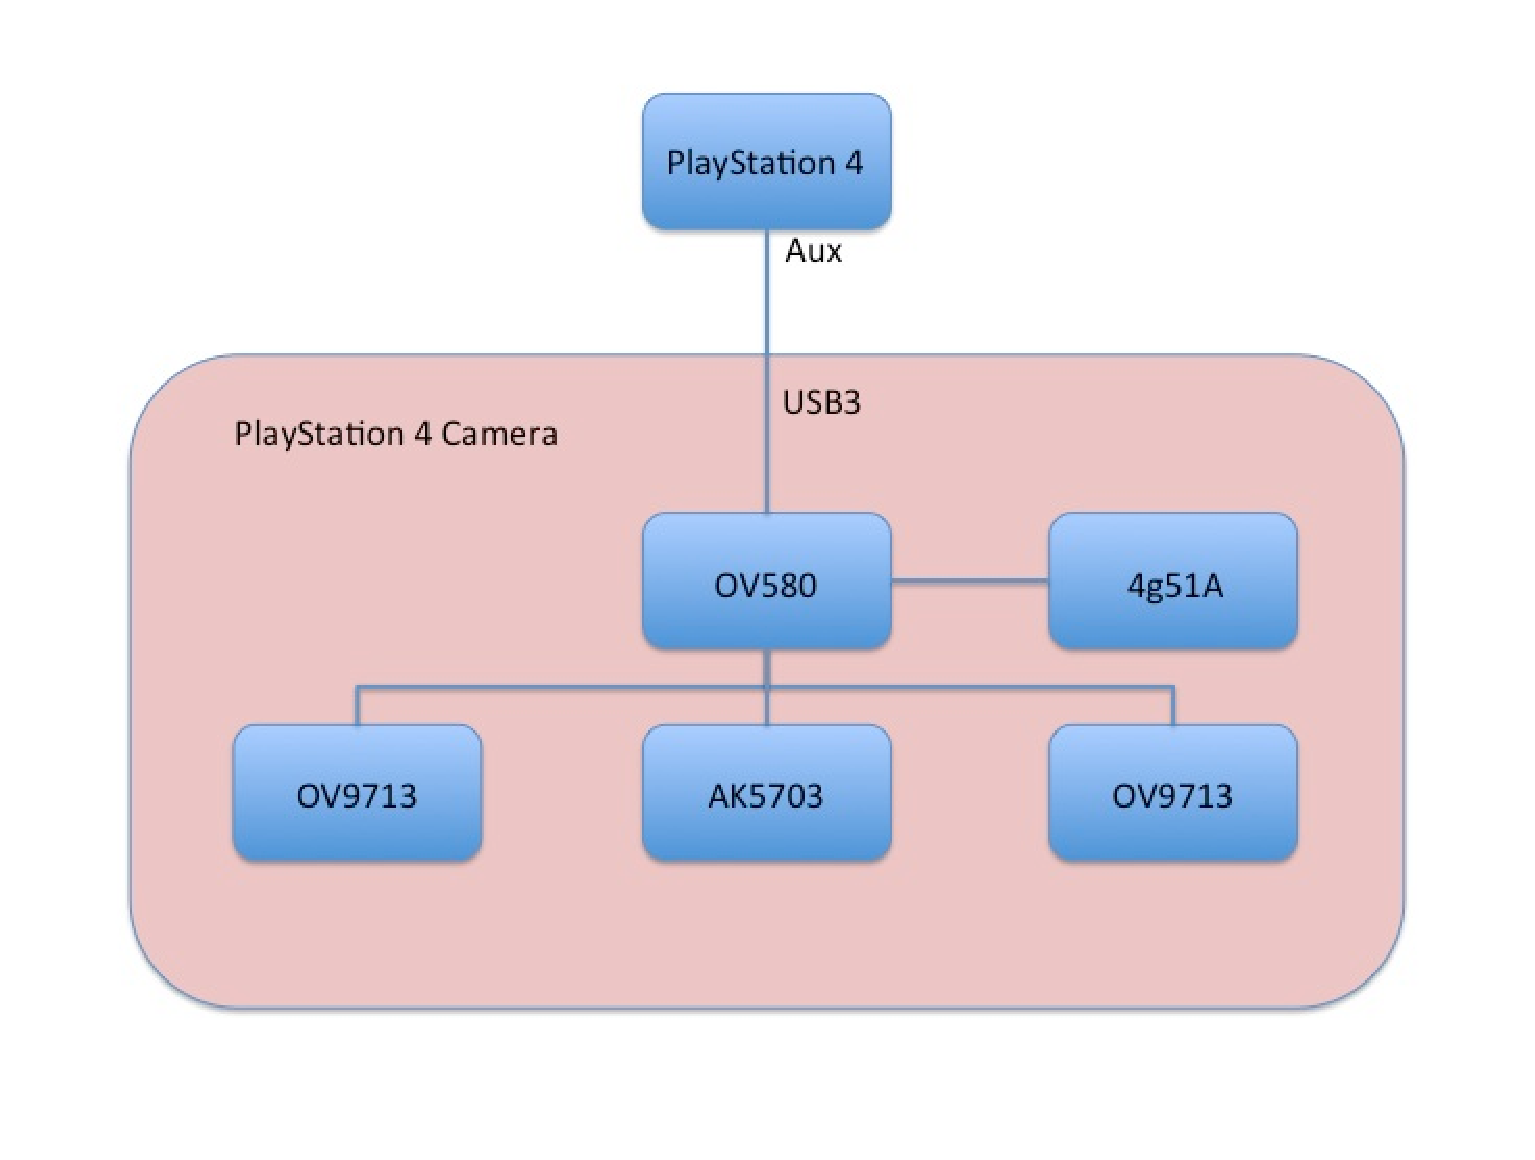
\includegraphics[width=0.9\textwidth]{images/cap3/PlaystationCameraDiagrama.eps}
    \captionof{figure}{Diagrama de PlayStation Camera}
    \label{fig:Playstation-Camera-Diagram}
\end{minipage}

Por su parte ña cámara cuenta con varios ajustes programables: exposición,
balanceo de blancos, gama, saturación, contraste, nitiddez y tono.

%+++++++++++++++++++++++++++++++++++++++++++++++++++++++++++++++++++++++++++++++
\begin{table}[!ht]
\begin{center}
\begin{tabular}{|p{60mm}|p{100mm}|} \hline 
\textbf{Nombre} & \textbf{Descripción} \\ \hline
Dimensiones
&
186mm x 27mm x 27mm
\\
\hline

Peso
&
183 gramos
\\
\hline

Conexión
&
USB 3.0 propietario
\\
\hline

Rango de captura
&
+30cm
\\
\hline

Campo de visión (FOV)
&
85º
\\
\hline

Apertura
&
f/2.0
\\
\hline

Formato de vídeo
&
RAW16/RAW8, YUV442/YUV8
\\
\hline

Profundidad de color
&
12-bit (4096 colores)
\\
\hline

Resolución
&
1280x800 @60FPS,
640x400 @120FPS,
320x200 @240FPS,
160x100 @240FPS,
\\
\hline

Micrófono
&
Multiarray de 4 canales
\\
\hline

\end{tabular}
\end{center}
\caption{Tabla resumen de las características de PlayStation Camera}
\label{table:playstation-camera}
\end{table}
%+++++++++++++++++++++++++++++++++++++++++++++++++++++++++++++++++++++++++++++++


%+++++++++++++++++++++++++++++++++++++++++++++++++++++++++++++++++++++++++++++++
